%\begin{frame}[fragile]{Why care about faster nearest neighbor queries?}
\begin{frame}[fragile]{Why care about cover trees?}
% image from: http://scikit-learn.org/0.11/auto_examples/neighbors/plot_classification.html

They speed up nearest neighbor queries, e.g. in
 $k$-nn classification:

\begin{center}
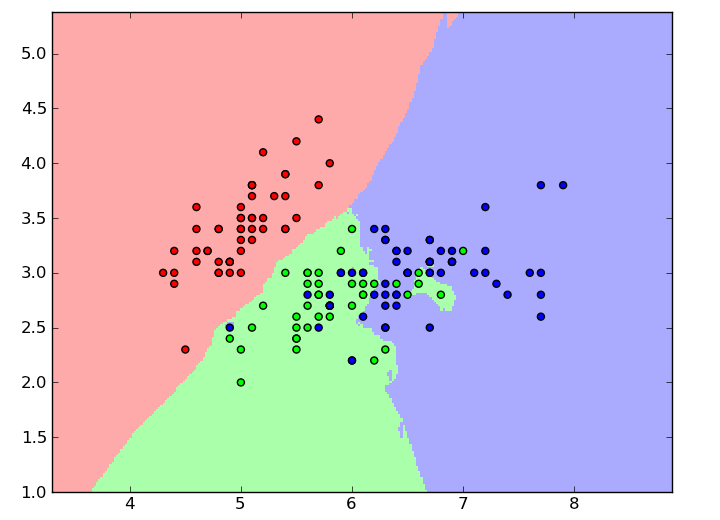
\includegraphics[width=5.5cm]{covertree/knn.png}
\end{center}
%source: scikit learn

But neighbor queries are used in many other algorithms too:
\begin{itemize}
\item Localized support vector machines (Segata \& Blanzieri, 2010)
\item Dimensionality reduction (Lisitsyn \emph{et. al.}, 2013)
\item Reinforcement learning (Tziortziotis \emph{et. al.}, 2014)
\end{itemize}

\vspace{0.05in}
{\tiny image from: \url{http://scikit-learn.org}}

\end{frame}

